\input{../header}

\begin{document}
%


%\onehalfspacing
\allowdisplaybreaks
%##################################################################
\section{PS\#1: Numerical integration - \red{Answer key} }

\begin{red}
(Note: I split the derivative review questions off into their own separate pdf.)
\end{red}

\begin{enumerate}[leftmargin=0pt]

\item Suppose $w(t)$ is a function modeling the weight of a puppy over the first year of its life. We'll say $w$ is measured in kg and is $t$ measured in months.
\begin{enumerate}
    \item (Dimensional analysis saves lives!) What are the units on $w'(t)$? Write a sentence or two explaining why.
    
    \begin{red}
    The units on $w'(t)$ will be kg/mo. This is because the units of the derivative are the units of the output (of the original function) per the units of the input. Since the units on $w(t)$ were kg, the units on $w'(t)$ are kg/mo.
    \end{red}
    \item Suppose that according to our model, $w'(t) = 4.7 \exp(-0.187t)$, and that the dog weighed 0.4kg when born. Draw this function on Desmos and scale your axes so that the graph goes pretty much from corner to corner of your viewing window.
    
    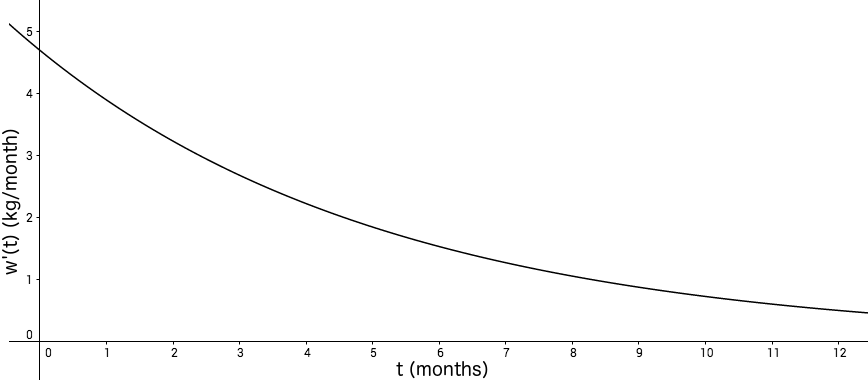
\includegraphics[width=0.7\textwidth]{../images/dog-weight/prelab.png}
    \item Draw four rectangles, evenly spaced in the domain, so that the top-\textbf{left} corner of each rectangle touches the graph and the base of the rectangle is on the $t$-axis. Label:
    \begin{itemize}
        \item the height of each rectangle (a number with units)
        \item the width of each rectangle (a number with units)
        \item the area of each rectangle (a number with units)
    \end{itemize}
    Use your labels to find the total area of all four rectangles (as a number with units).
    
    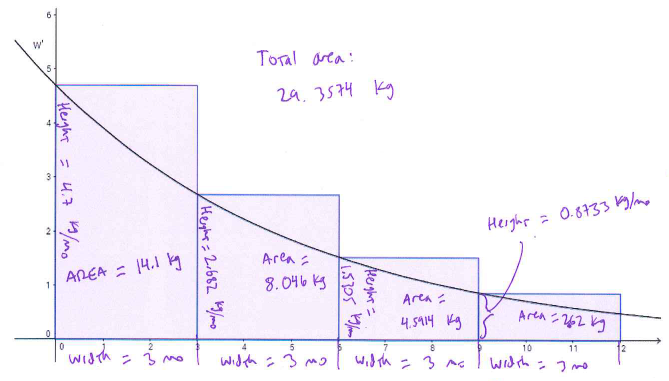
\includegraphics[width=0.95\textwidth]{../images/dog-weight/left-ans.png}
    \item Now do the same, but with the top-\textbf{right} corner of each rectangle touching the graph. Same labeling instructions.
    
    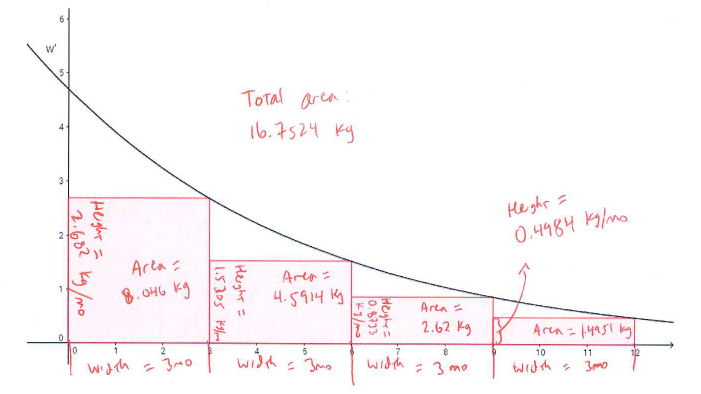
\includegraphics[width=0.95\textwidth]{../images/dog-weight/right-ans.png}
    \item Use your calculations to produce a reasonable estimate of the weight of the dog on its birthday. Explain why your estimate is good. (Don't forget the 0.4kg birth weight!)
    
    \begin{red}
    The area under the graph of $w'(t)$ from $t = 0$ to $12$ is the amount of weight the dog \textbf{gains} during her first year. Therefore, in order to obtain the dog’s actual \textbf{weight} at the end of one year, we must add the birth weight of 0.4 kg to the value we obtain through our Riemann sums.
    
    One reasonable guess is from the left sum: birthday weight $\approx \SI{29.36}{kg} + \SI{0.4}{kg} = \SI{29.76}{kg}$.
    
    A different reasonable guess is from the right sum: birthday weight $\approx \SI{16.75}{kg} + \SI{0.4}{kg} = \SI{17.15}{kg}$.
    
    To make a better guess, we might notice that the left sum is certainly an overestimate of the growth, whereas the right sum is certainly an underestimate of the growth. Therefore we can use the average of those two sums as a more accurate guess for how much the dog grew:
    \[\text{birthday weight } \approx \frac{\SI{29.36}{kg}+ \SI{16.75}{kg}}{2} + \SI{0.4}{kg} \approx \SI{23.06}{kg} + \SI{0.4}{kg} = \SI{23.46}{kg}.\]
    
    You may have a different strategy for coming up with weight estimates, and that's both good and cool!
    \end{red}
\end{enumerate}

\end{enumerate}
\end{document}